\lecture{23}{Maxwell Distribution, Partition Functions and Free Energy}{Qiang Zhu}{scribe-name1,2,3}
%\footnotetext{These notes are partially based on those of Nigel Mansell.}
% **** YOUR NOTES GO HERE:
% Some general latex examples and examples making use of the
% macros follow.  
%**** IN GENERAL, BE BRIEF. LONG SCRIBE NOTES, NO MATTER HOW WELL WRITTEN,
%**** ARE NEVER READ BY ANYBODY.

\section{Maxwell Speed Distribution}
In the very first lecture, we briefly mentioned a microscopic model to link the speed of particles to the temperature,
\begin{equation} \label{PV-micro} PV = Nm{\overline v_x^2} = NkT\end{equation}

But this is just a sort of average. Technically, the speeds of particles should follow some distribution.
Let's call it as $D(v)$. What's the dependence of $D(v)$?

The first factor should be just the Boltzmann factor. 
\begin{equation}
D(v) \propto e^{E/kT} = e^{-mv^2/2kT}
\end{equation}
This only accounts for ideal gas, where the transnational motion is independent of other variables.

The second factor should be the velocity space. For a give $v$, it could be in any directions. The the space is $4\pi v^2$.
Therefore,
\begin{equation}
D(v) = C \cdot 4\pi v^2 e^{-mv^2/2kT}
\end{equation}

Where $C$ is a constant. According to 
\begin{equation}
1 = \int _0 ^{\infty} D(v)dv  = C \cdot 4\pi v^2 e^{-mv^2/2kT} dv
\end{equation}

Changing variables to $x = v\sqrt{m/2kT}$,
\begin{equation}
1 =  4\pi C (\frac{2kT}{m})^{3/2}  \int _0 ^{\infty} x^2 e^{-x^2} dx
\end{equation}

By using some trick, you can find
\begin{equation}
\int _0 ^{\infty} x^2 e^{-x^2} dx = \sqrt{\pi}/4
\end{equation}

Therefore, $C=(m/2\pi kT)^{3/2}$.

Our final results is therefore,
\begin{equation}
D(v) = (\frac{m}{2\pi kT})^{3/2}4\pi v^2 e^{-mv^2/2kT}
\end{equation}

\begin{figure}[h]
\centering
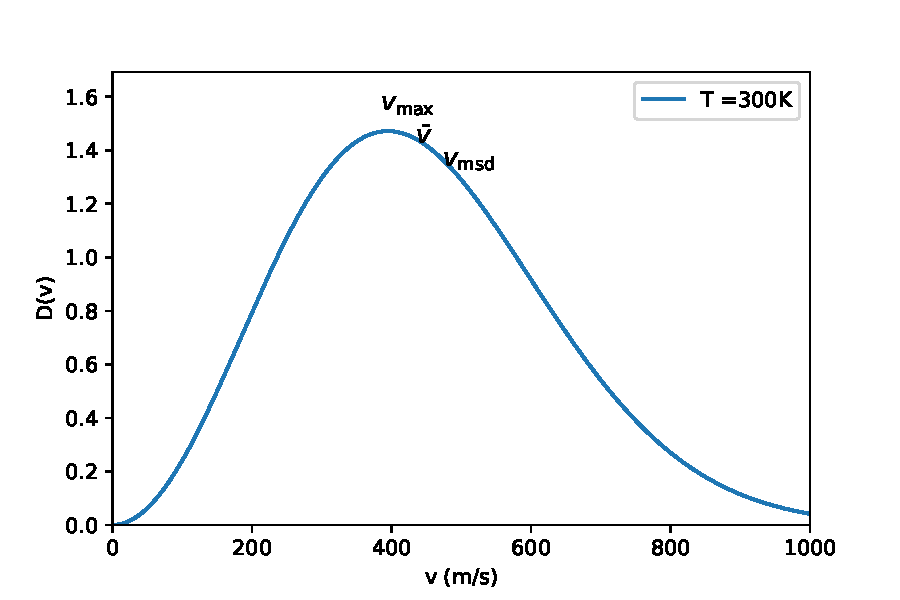
\includegraphics[width=10cm]{imgs/Maxwell-speed.pdf}
\caption{The Maxwell speed distribution and different types of characteristic speeds. }
\end{figure}




The average speed:
\begin{equation}
\bar{v} = \int _0 ^{\infty} vD(v) dv = \sqrt{\frac{8kT}{\pi m}}
\end{equation}

The rms speed:
\begin{equation}
\bar{v^2} = \int_0^{\infty} v^2D(v) dv = 3kT/m
\end{equation}

The most likely speed:
\begin{equation}
\frac{\partial D(v)}{\partial v} = 0 ~~~~\rightarrow~~~~~~ v_\text{max}= \sqrt{\frac{2kT}{m}}
\end{equation}


\section{Partition Function and Free Energy}
For a system in equilibrium with a reservoir at temperature $T$, the quantity most analogous to $\Omega$
is $Z$. Does the natural logarithm of $Z$ has some meaning?

Recall the definition of $F = U - TS$, the partial derivative with respect to $T$ is
\begin{equation}
(\frac{\partial F}{\partial{T}})_{V,N} = -S = \frac{F-H}{T}
\end{equation}

This is a differential equation for the function $F(T)$, for any given $V$ and $V$. If we use $\bar{F}$ to 
express the $kT\text{ln}Z$, then
\begin{equation}
\frac{\partial{\bar{F}}}{\partial T} = \frac{\partial}{\partial T}(-kT\text{ln}Z) = -k\text{ln}Z - kT \frac{\partial}{\partial T}\text{ln}Z
\end{equation}

In the 2nd term, we rewrite it in terms of $\beta=1/kT$
\begin{equation}
\frac{\partial}{\partial T}\text{ln}Z = \frac{\partial{\beta}}{\partial T} \frac{\partial}{\partial T}\text{ln}Z 
                                      = \frac{-1}{kT^2} \frac{1}{Z} \frac{\partial Z}{\partial {\beta}} 
                                      = \frac{U}{kT^2}
\end{equation}
Therefore,

\begin{equation}
\frac{\partial{\bar{F}}}{\partial T} = -k\text{ln}Z - kT \frac{U}{kT^2} = \frac{\bar{F}-U}{T}
\end{equation}

Therefore, $\bar{F}$ obeys the exactly same differential equation as $F$.

At $T$=0, the original $F$ is simply equal to $U$, the energy must be the lowest possible energy $U_0$, since the Boltzmann
factors for all excited states will be infinitely suppressed in comparison to the ground state. Therefore,
\begin{equation}
\bar{F}(0)= -kT\text{ln}Z(0)= U(0) = F(0)
\end{equation}

This relation could be very useful to compute entropy, pressure, and so on.
\begin{equation}
S = -(\frac{\partial{F}}{\partial{T}})_{V,N} ~~~~  P = -(\frac{\partial{F}}{\partial{T}})_{T,N} 
~~~~~~ \mu = (\frac{\partial{F}}{\partial{N}})_{V,T}
\end{equation}


